%% Beispiel-Präsentation
\documentclass[en]{sdqbeamer}
 
 % Eigene packages
\usepackage{verbatim}
\usepackage{longtable}
 
%% Titelbild
\titleimage{bauplan_2020_sdq}

%% Gruppenlogo
\grouplogo{sdq_logo.pdf} 

%% Gruppenname
\groupname{Institute for Program Structures and Data Organization (IPD)}

% Beginn der Präsentation

\title[Tuning of XAI tools]{Tuning of Explainable Artificial Intelligence tools in the field of text analysis}
%\subtitle{entsprechend den Gestaltungsrichtlinien vom 1. August 2020}
\author[Philipp Weinmann]{Philipp Weinmann}

\date[11.\,06.\,2021]{11. Juni 2021}

% Literatur 
 
 \usepackage[citestyle=numeric,style=numeric,backend=biber]{biblatex}
%\usepackage[citestyle=authoryear,bibstyle=numeric,hyperref,backend=biber]{biblatex}
\addbibresource{presentation.bib}
\bibhang1em

\hypersetup{colorlinks,linkcolor={blue},citecolor={blue},urlcolor={blue}}  

\begin{document}

%Titelseite
\KITtitleframe


%Inhaltsverzeichnis
\begin{frame}{Inhaltsverzeichnis}
\tableofcontents
\end{frame}

\section{Motivation}

\begin{large}

% Xai in general
\begin{frame}{Motivation: XAI in general}
\begin{center}
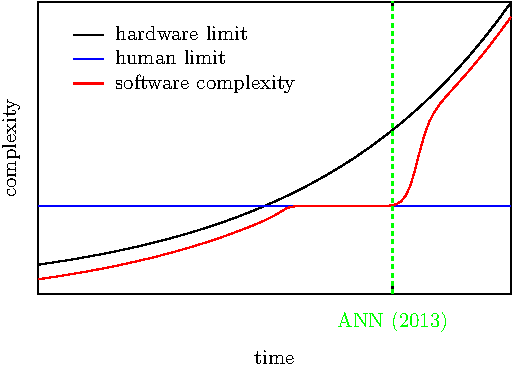
\includegraphics[width=0.5\linewidth]{images/Complexity.pdf}\\
\end{center}
\end{frame}

% Three scenarios

\begin{frame}{Motivation: XAI in general}
\textbf{XAI can be used to:} 
\begin{enumerate}
    % Developers need a hint on how to solve a problem  without the use of artificial neural networks.
    \item provide a hint to solve the problem without ANN
    \pause
    % We understand a fraction of how the artificial intelligence makes a decision but it is enough to disqualify it. This is especially important if some unwanted behaviour like biased \textit{(racist/sexist/...)} decisions are revealed.
    \item disqualify
    \pause
    % We understand a fraction of how the artificial intelligence makes a decision and the approach feels plausible to humans.
    \item increase trust
\end{enumerate}
\end{frame}

% Tools for XAI

\section{Related Works}

\iffalse
% Hard to categorize
% sentence to each approach
\begin{frame}{Related Works}
    \begin{itemize}
        \item Perturbation based approaches
        \item Function based approaches
        \item Surrogate-/ Sampling based approaches
        \item Structure-based approaches
    \end{itemize}
\end{frame}
\fi


\section{Interpretability} % Basics: Interpretability

% Interpretability
%% Transparency, Decomposability, Algorithmic transparency
\begin{frame}{Interpretability}
    \begin{itemize}
        \item Simulatability
        \pause
        \item Decomposability
        \pause
        \item Algorithmic transparency
    \end{itemize}
    \cite{lipton2017mythos} \\
    \pause
    => need for an explanation model
\end{frame}



\begin{frame}{Interpretability: Example}
    % Example of where interpretability does not work

    \begin{center}
            \begin{tabular}{c|c}
                Feature name & Feature importance \\ \hline
                rutgers & 0.040224 \\
                athos & 0.036232 \\
                geneva & 0.030274 \\
                1993 & 0.025009 \\
                christ & 0.022898 \\
                article & 0.021479 \\
                writes & 0.019735 \\
                com & 0.019473 \\
                paul & 0.016807 \\
                don't & 0.014403
            \end{tabular}
    \end{center}
\end{frame}

\iffalse
% second page of results
\begin{frame}{Interpretability: Example}
    % Example of where interpretability does not work

    \begin{center}
        \begin{tabular}{c|c}
            Feature name & Feature importance \\ \hline
            nntp-posting-host & 0.010084 \\
            atheism & 0.008166 \\
            christian & 0.00862 \\
            christianity & 0.008166 \\
            christians & 0.00797
        \end{tabular}
    \end{center}
\end{frame}
\fi

\section{Shap}

\begin{frame}
    \begin{figure}[H]
    \centering
    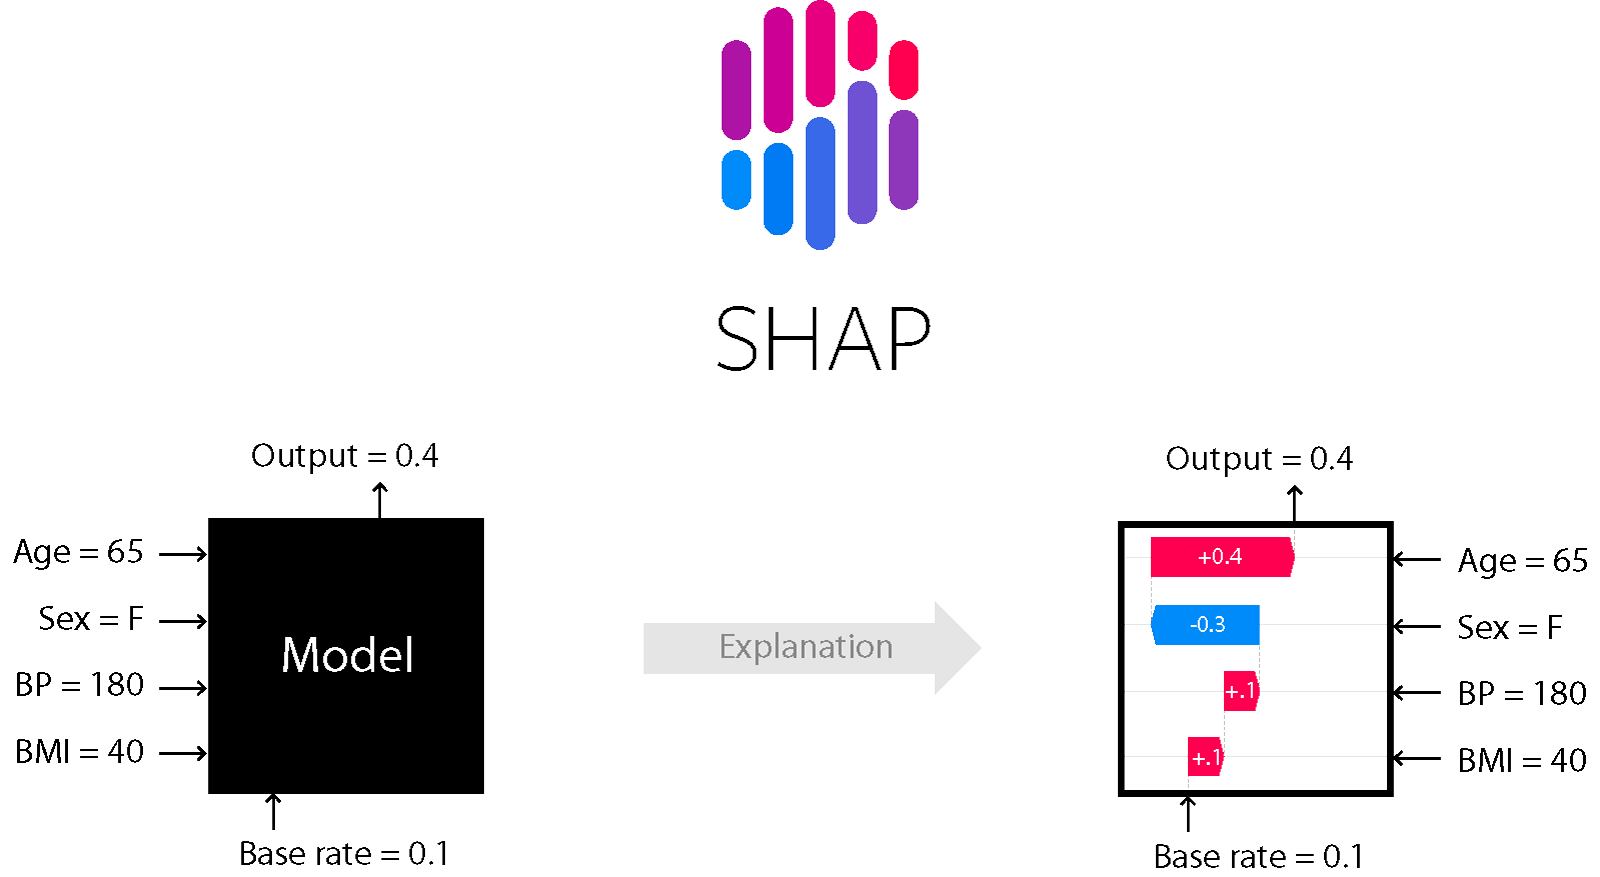
\includegraphics[width=\linewidth,height=0.8\textheight,keepaspectratio]{images/ShapExplanationVisualized.png}
    \caption{Visualization of a shap explanation \cite{shapDocs}}
    \label{fig:shap_visualization}
\end{figure}
\end{frame}

\begin{frame}{Shap: Competitive Game theory}
% Competitive Game Theory: very short
    \begin{figure}[H]
    \centering
    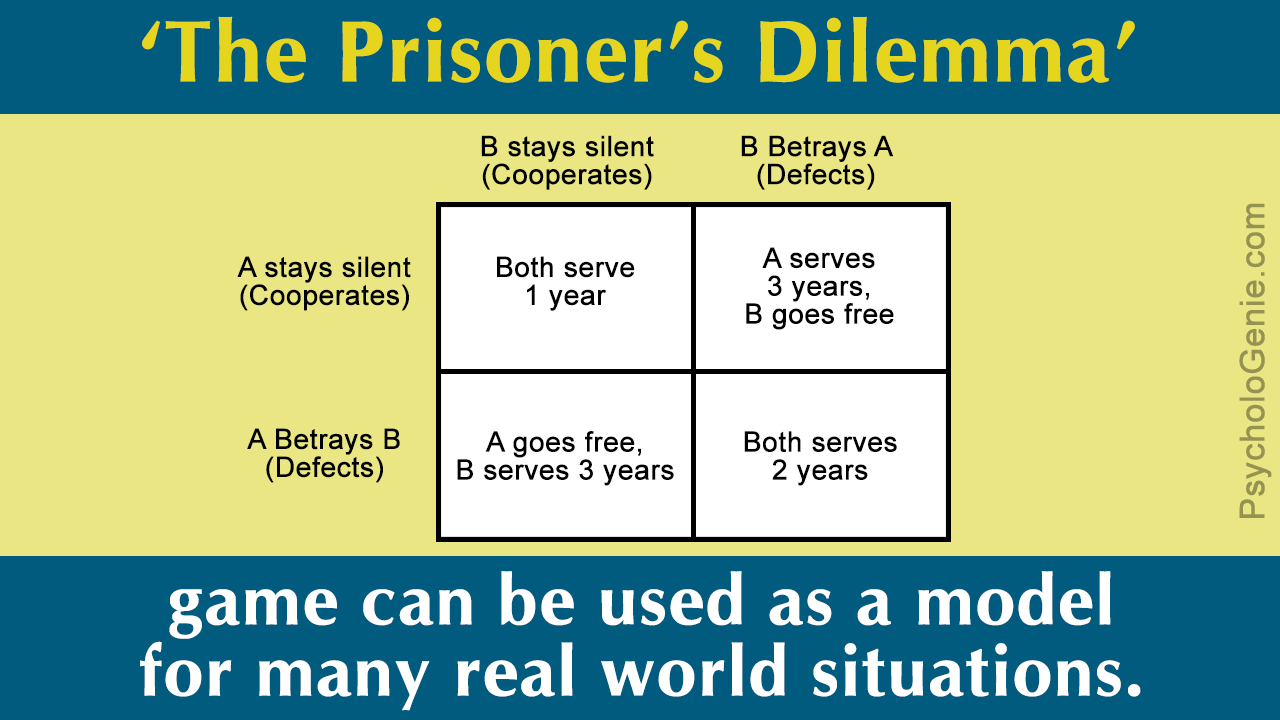
\includegraphics[width=\linewidth,height=0.6\textheight,keepaspectratio]{images/Prisoners dilemma.png}
    \caption{Prisoners Dilemma \cite{psychologenie_2014}}
    \label{fig:prisonersDilemma}
\end{figure}

\end{frame}

\begin{frame}{Competitive Game theory: text example}
    \begin{itemize}
        \item \enquote{\textbf{Jesus} word is the word of God} => 100\% christian
        \item \enquote{word is the word of God} => 100\% christian
        \vspace{1cm}
        \pause
        \item \enquote{word is the word of}
    \end{itemize}
\end{frame}

\iffalse
\begin{frame}{Shapley Properties}
\begin{itemize}
    \item Local Accuracy
    \item Missingness
    \item Consistency
\end{itemize}
\end{frame}
\fi

\section{Dataset}

\begin{frame}{Our Dataset}
\begin{itemize}
    \item 20Newsgroups\cite{Newsgroups20}: Atheist and Christian emails.
    \item Binary tfidf-classifier
\end{itemize}

\end{frame}

\section{Results}

\iffalse
% Dimensions of the explanation quality
\begin{frame}{Results: Explanation quality dimensions}
    \begin{itemize}
        \item Accuracy
        \item Interpretability
        \item Resource-requirements
    \end{itemize}
\end{frame}
\fi

% Our parameter
\begin{frame}[fragile]{Results: Parameter}
\begin{table}[H]
    \centering
    \begin{tabular}{c}
         \textbf{Text-Hierarchy}\\ \hline
         Word\\
         Sentence\\
         Paragraph\\
         2-gram\\
         ...
    \end{tabular}
    \caption{Parameter: Text Hierarchies}
    \label{tab:textHierarchies}
\end{table}
\end{frame}

\begin{frame}{Results: Parameter}
    \begin{figure}
        \centering
        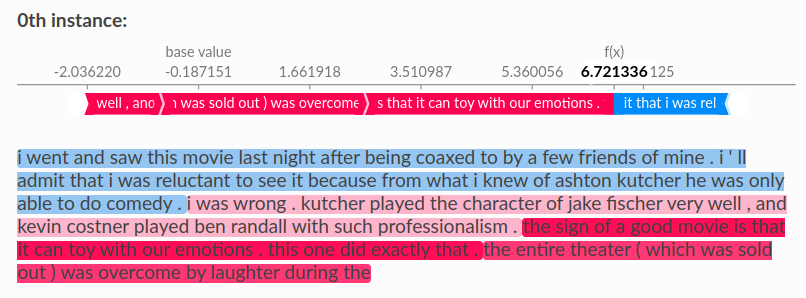
\includegraphics[width=\linewidth,height=0.6\textheight,keepaspectratio]{images/Sentence_XAI.png}
        \caption{Explanation with different text hierarchy example\cite{shapDocs}.}
        \label{fig:SentenceExplanation}
    \end{figure}
\end{frame}

\begin{frame}{Results: Calculation method}
\begin{exampleblock}{Context Influence}
\begin{center}
$contextInfluence(w’) = | classificationScore(W) - classificationScore(W\backslash w') - shapFeatureImportance(w') |$
\end{center}
\end{exampleblock}
\vspace{1cm}
\textcolor{gray}{
$classificationScore(W)$: The classification score the classifier gives the text W\\
\textit{$classificationScore(W \backslash w')$: The value the classifier gives the text W without the word w'}\\
\textit{$shapFeatureImportance(w')$: The feature importance shap gives to the word w'}\\
\textit{$contextInfluence(w')$: The importance of the context of the word w' according to shap}}
\end{frame}

\iffalse
% Our Results
\begin{frame}{Results: Calculation method}
    \begin{enumerate}
        \item We classify our corpus and get a Classification score $C_1$
        \item We extract the influence $I_i$ shap gives each feature i.
        \item We classify our corpus without a single feature $F_i$ (which had influence $I_i$ according to shap) and get Classification score $C_2$
        \item We calculate the absolute difference between the influence $I_i$ and the difference in classification scores : ($C_1 - C_2$). Let's call that Difference $D_i$.
        \item After repeating these steps for n features $F_i$, we calculate the average of the absolute of these differences \[D_{avg} =  \frac{1}{n}\sum_{i=1}^{n} |D_i|\]
        \item We plot $D_{avg}$ for each text hierarchy
    \end{enumerate}
\end{frame}
\fi
\begin{frame}
    \begin{figure}[H]
        \centering
        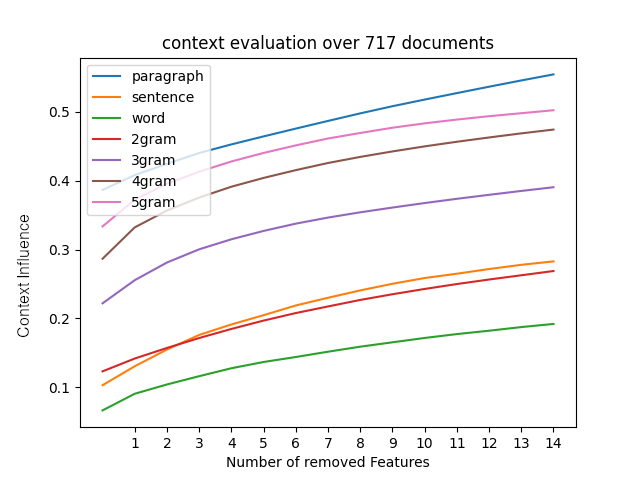
\includegraphics[width=\linewidth,height=\textheight,keepaspectratio]{images/clemensEvalPlotAllSelectedDocsCombinedYAXIS.png}
    \end{figure}
\end{frame}


% Recommendation for XAI users
\begin{frame}{Results: Recommendation}
    \begin{itemize}
        \item Stop using words in XAI while using shap, try to use grammatical constructs like sentences: Our data shows a decrease by 89,33\% of the context-influence per word presented to the user.
    \end{itemize}
\end{frame}

\iffalse
\begin{frame}{Critique}
    \begin{itemize}
        \item Emails too short to analyse paragraphs
        \item Dataset too small
        \item Missing error bar
    \end{itemize}
\end{frame}
\fi

\section{Framework}
% Overview of the Framework
% Intended use

\begin{frame}
    \begin{figure}[H]
            \centering
            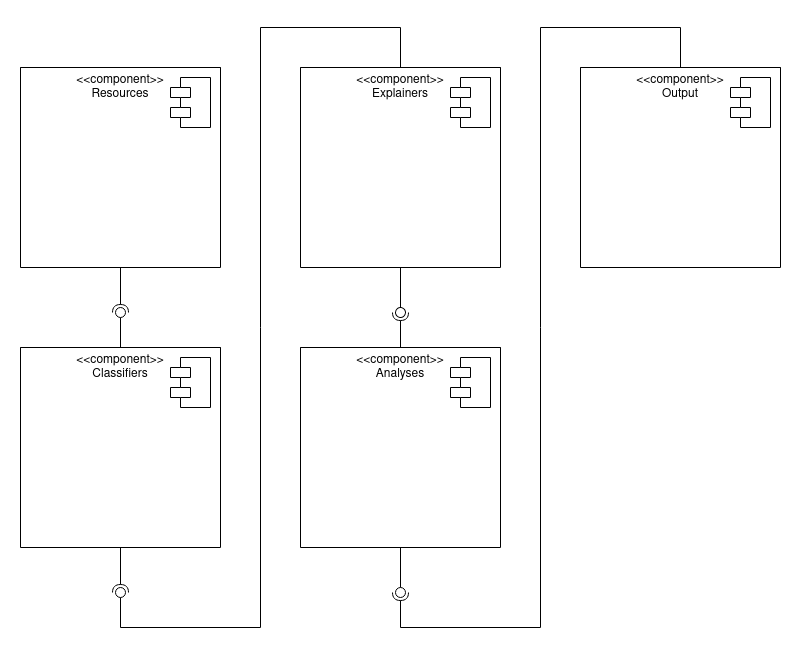
\includegraphics[width=\linewidth,height=0.85\textheight,keepaspectratio]{images/Copy of Component_diagram_overview_framework_flatter.png}
            \caption{Framework overview}
    \end{figure}
\end{frame}



\section{Outlook}

% Interactivity
\begin{frame}[plain]
        \begin{figure}[H]
            \centering
            
\includegraphics[width=\linewidth,height=0.9\textheight,keepaspectratio]{images/Interactivity.jpg}
            \caption{Outlook: Interactivity \cite{das_2021}}
    \end{figure}
\end{frame}

% How do I remove these frames from navbar?!

\begin{frame}
  \centering \Huge
  \emph{Thank you for listening}
\end{frame}

\begin{frame}{References}

\printbibliography
\end{frame}

\end{large}



\end{document}